\section{VPN on Ubuntu}

If you use Ubuntu as your operating system, you can connect to a VPN by
using the built-in \emph{NetworkManager}. This application is able to
set up networks with OpenVPN. PPTP should not be used for security
reasons. Unfortunately at the time of writing a L2TP interface is not
available in Ubuntu. (It can be done manually, but it goes beyond the
scope of this document).

The following example will explain how to connect with an
OpenVPN-server. Under all situations we assume you already have a VPN
account as described earlier in this section.

\subsection{Preparing Network Manager for VPN networks}

For Ubuntu there is an excellent network utility: Network Manager. This
is the same utility you use to set up your Wireless (or wired) network
and is normally in the upper right corner of your screen (next to the
clock). This tools is also capable of managing your VPNs, but before it
can do so, it's necessary to install some extensions.

\subsubsection{Installing OpenVPN extension for Network Manager}

To install the plugins for Network Manager we will use the Ubuntu
Software Center.

\begin{enumerate}[1.]
\item
  Open the Ubuntu Software Center by typing software in the Unity search
  bar
\end{enumerate}
\begin{figure}[htbp]
\centering
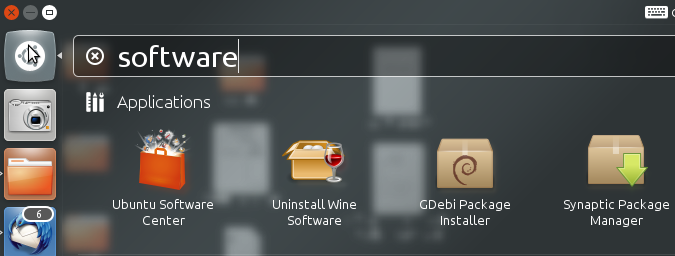
\includegraphics{vpn_ubuntu_001.png}
\caption{VPN on Ubuntu}
\end{figure}

\begin{enumerate}[1.]
\setcounter{enumi}{1}
\item
  The Ubuntu Software Center enables you to search, install and remove
  software on your computer. Click on the search box at the top right of
  the window.
\end{enumerate}
\begin{figure}[htbp]
\centering
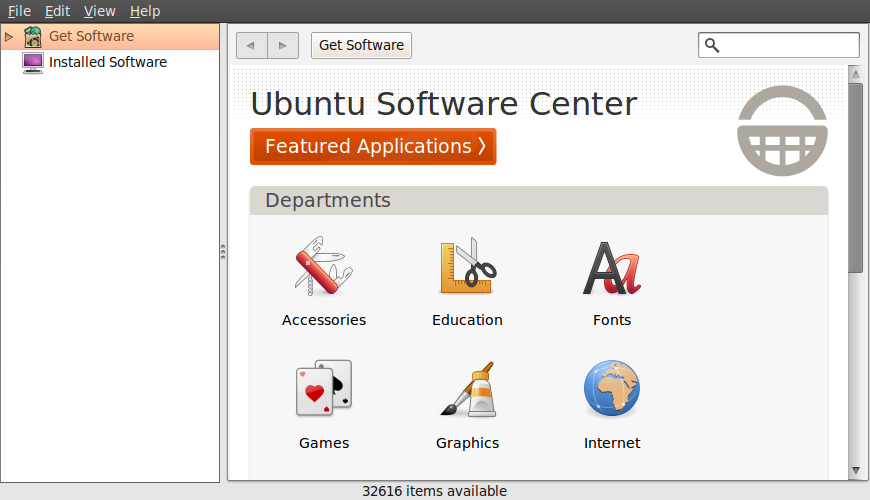
\includegraphics{vpn_ubuntu_002.png}
\caption{VPN on Ubuntu}
\end{figure}

\begin{enumerate}[1.]
\setcounter{enumi}{2}
\item
  In the search box, type in ``network-manager-openvpn-gnome'' (which is
  the extension that will enable OpenVPN). It's necessary to type the
  full names because the packages are classified as ``technical'' and
  don't pop-up earlier. These packages include all the files you need to
  establish a VPN connection successfully.
\end{enumerate}
\begin{figure}[htbp]
\centering
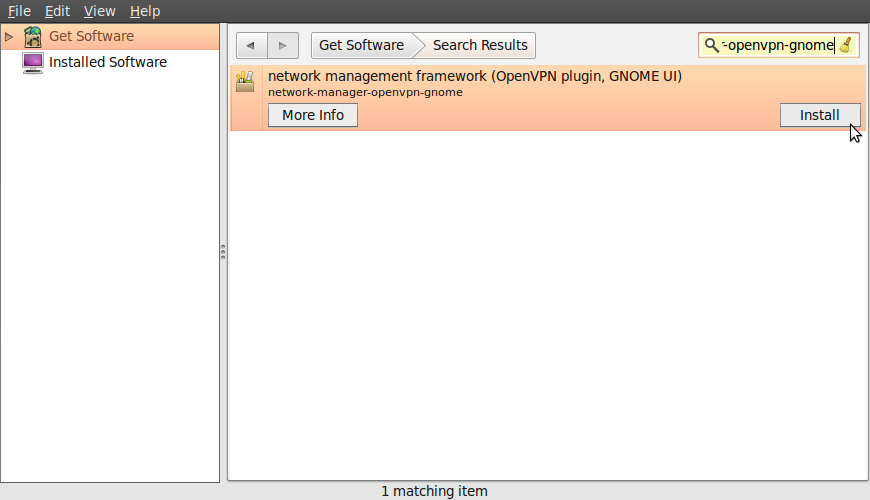
\includegraphics{vpn_ubuntu_003.png}
\caption{VPN on Ubuntu}
\end{figure}

\begin{enumerate}[1.]
\setcounter{enumi}{3}
\item
  Ubuntu may ask you for additional permissions to install the program.
  If that is the case, type in your password and click Authenticate.
  Once the package is installed, you can close the Software Center
  window.
\end{enumerate}
\begin{figure}[htbp]
\centering
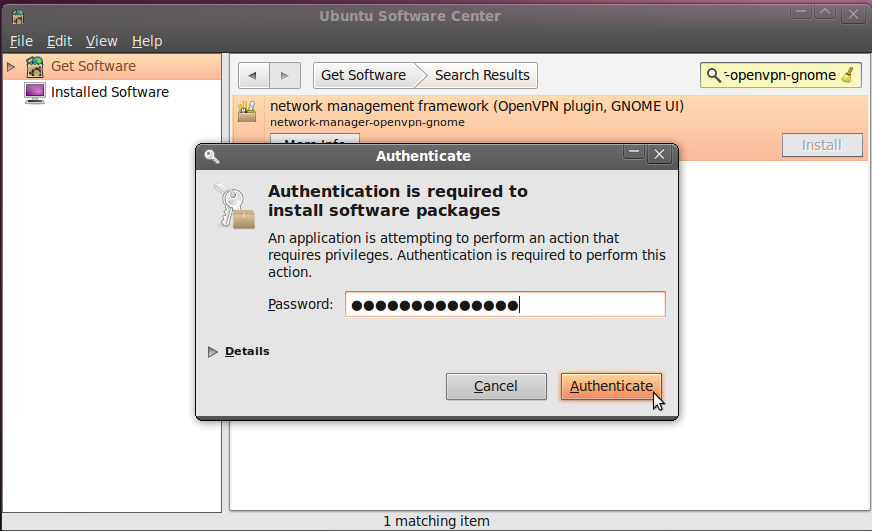
\includegraphics{vpn_ubuntu_004.png}
\caption{VPN on Ubuntu}
\end{figure}

\begin{enumerate}[1.]
\setcounter{enumi}{4}
\item
  To check if the extensions are correctly installed, click on the
  NetworkManager (the icon at the left of your system clock) and select
  VPN Connections \textgreater{} Configure VPN.
\end{enumerate}
\begin{figure}[htbp]
\centering
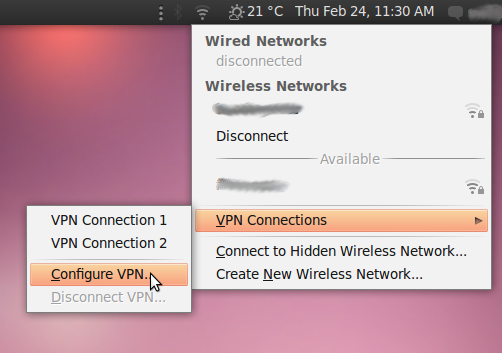
\includegraphics{vpn_ubuntu_005.png}
\caption{VPN on Ubuntu}
\end{figure}

\begin{enumerate}[1.]
\setcounter{enumi}{5}
\item
  Click Add under the VPN tab.
\end{enumerate}
\begin{figure}[htbp]
\centering
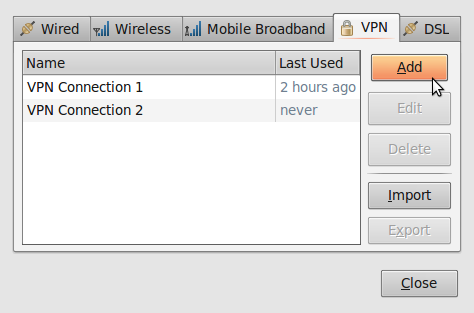
\includegraphics{vpn_ubuntu_006.png}
\caption{VPN on Ubuntu}
\end{figure}

\begin{enumerate}[1.]
\setcounter{enumi}{6}
\item
  If you see a pop-up asking for the type of VPN and the tunnel
  technology (OpenVPN) option is available, this means that you have
  installed the VPN extension in Ubuntu correctly. If you have your VPN
  login information ready, you can continue right away, else you first
  have to get a VPN account from a VPN-provider. If this is the case,
  click cancel to close the Network Manager.
\end{enumerate}
\begin{figure}[htbp]
\centering
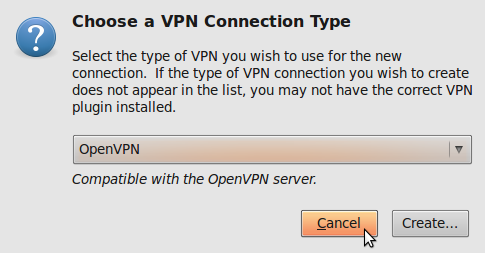
\includegraphics{vpn_ubuntu_007.png}
\caption{VPN on Ubuntu}
\end{figure}

\subsection{Configuring an OpenVPN network}

Let's assume you received your configuration files and credentials from
your VPN provider. This information should contain the following

\begin{itemize}
\item
  an *.ovpn file, ex. air.ovpn
\item
  The file: ca.crt (this file is specific for every OpenVPN provider)
\item
  The file: user.crt (this file is your personal certificate, used for
  encryption of data)
\item
  The file: user.key (this file contains your private key. It should be
  protected in a good manner. Losing this file will make your connection
  insecure)
\end{itemize}
In most cases your provider will send these files to you in a zip file.
Some openvpn providers use username and password authentication which
will not be covered.

\begin{enumerate}[1.]
\item
  Unzip the file you have downloaded to a folder on your hard drive
  (e.g.: ``/home/{[}yourusername{]}/.vpn''). You should now have four
  files. The file ``air.ovpn'' is the configuration file that you need
  to import into NetworkManager.
\end{enumerate}
\begin{figure}[htbp]
\centering
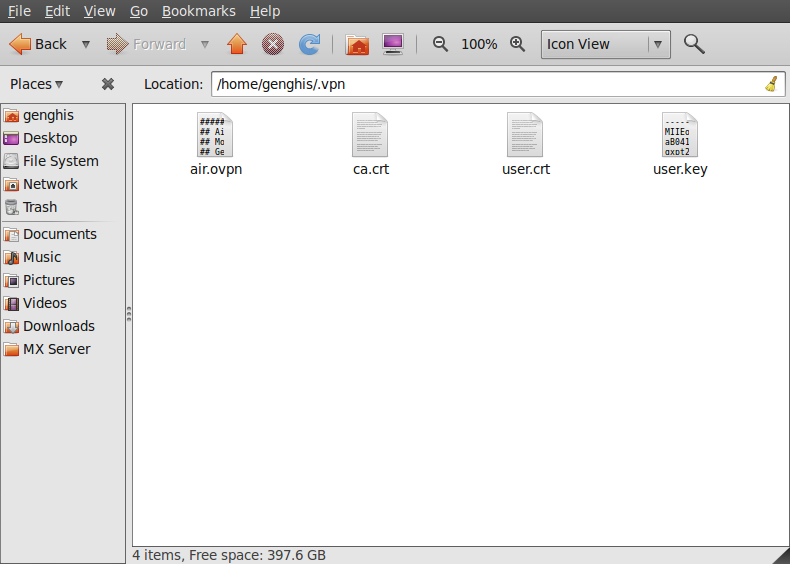
\includegraphics{vpn_ubuntu_008.png}
\caption{VPN on Ubuntu}
\end{figure}

\begin{enumerate}[1.]
\setcounter{enumi}{1}
\item
  To import the configuration file, open NetworkManager and go to VPN
  Connections \textgreater{} Configure VPN.
\end{enumerate}
\begin{figure}[htbp]
\centering
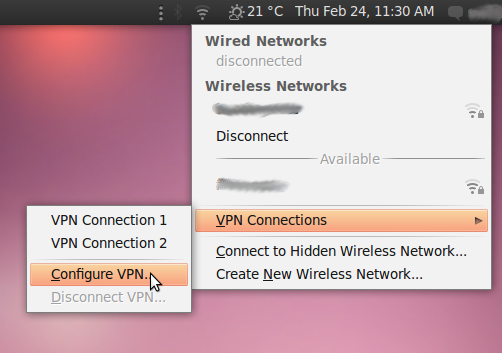
\includegraphics{vpn_ubuntu_009.png}
\caption{VPN on Ubuntu}
\end{figure}

\begin{enumerate}[1.]
\setcounter{enumi}{2}
\item
  Under the VPN tab, click Import.
\end{enumerate}
\begin{figure}[htbp]
\centering
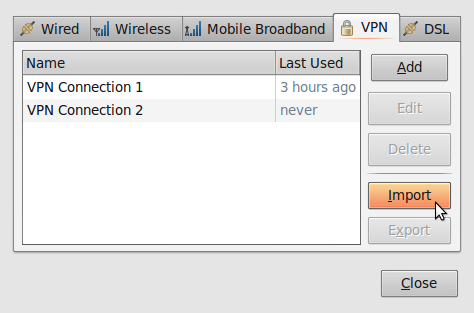
\includegraphics{vpn_ubuntu_010.png}
\caption{VPN on Ubuntu}
\end{figure}

\begin{enumerate}[1.]
\setcounter{enumi}{3}
\item
  Locate the file air.ovpn that you have just unzipped. Click Open.
\end{enumerate}
\begin{figure}[htbp]
\centering
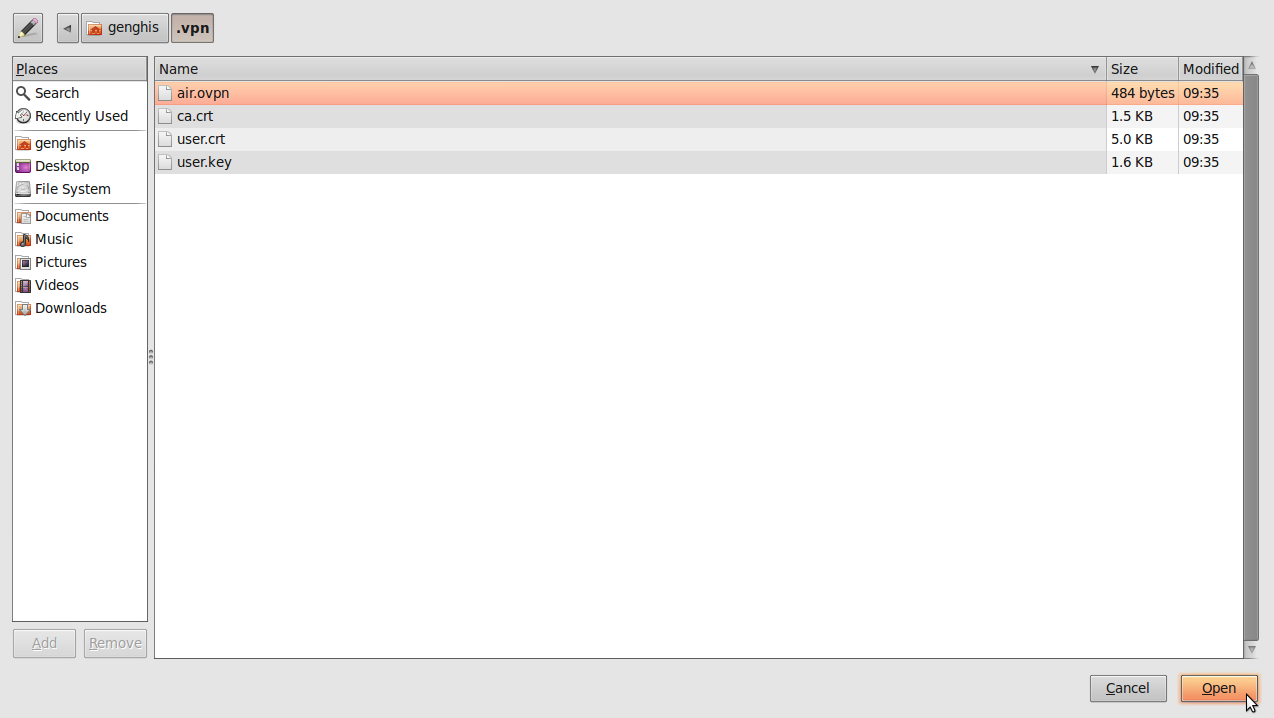
\includegraphics{vpn_ubuntu_011.png}
\caption{VPN on Ubuntu}
\end{figure}

\begin{enumerate}[1.]
\setcounter{enumi}{4}
\item
  A new window will open. Leave everything as it is and click Apply.
\end{enumerate}
\begin{figure}[htbp]
\centering
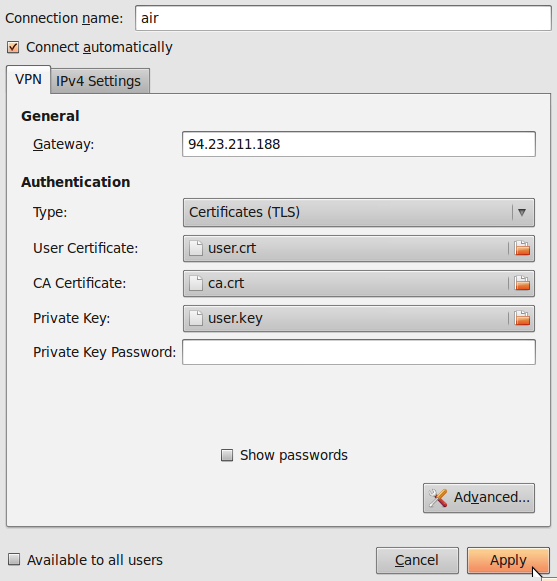
\includegraphics{vpn_ubuntu_012.png}
\caption{VPN on Ubuntu}
\end{figure}

\begin{enumerate}[1.]
\setcounter{enumi}{5}
\item
  Congratulations! Your VPN connection is ready to be used and should
  appear on the list of connections under the VPN tab. You can now close
  NetworkManager.
\end{enumerate}
\begin{figure}[htbp]
\centering
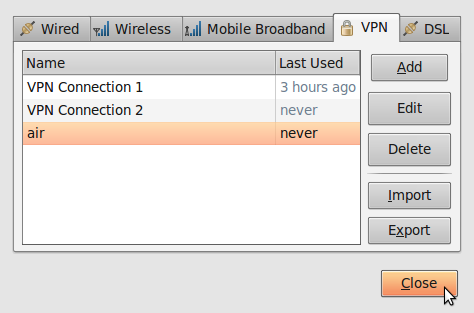
\includegraphics{vpn_ubuntu_013.png}
\caption{VPN on Ubuntu}
\end{figure}

\subsection{Using your new VPN connection}

Now that you configured NetworkManager to connect to a VPN service using
the OpenVPN client, you can use your new VPN connection to circumvent
Internet censorship. To get started, follow these steps:

\begin{enumerate}[1.]
\item
  In the NetworkManager menu, select your new connection from VPN
  Connections.
\end{enumerate}
\begin{figure}[htbp]
\centering
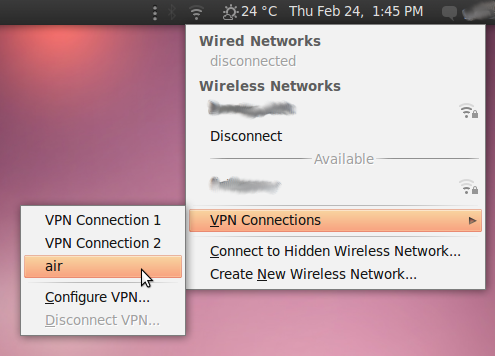
\includegraphics{vpn_ubuntu_014.png}
\caption{VPN on Ubuntu}
\end{figure}

\begin{enumerate}[1.]
\setcounter{enumi}{1}
\item
  Wait for the VPN connection to be established. When connected, a small
  padlock should appear right next to your NetworkManager icon,
  indicating that you are now using a secure connection. Move your
  cursor over the icon to confirm that the VPN connection is active.
\end{enumerate}
\begin{figure}[htbp]
\centering
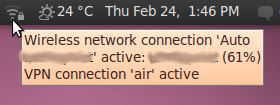
\includegraphics{vpn_ubuntu_015.png}
\caption{VPN on Ubuntu}
\end{figure}

\begin{enumerate}[1.]
\setcounter{enumi}{2}
\item
  Test your connection, using the method described in the ``Make sure it
  works'' section of this chapter.
\item
  To disconnect from your VPN, select VPN Connections \textgreater{}
  Disconnect VPN in the NetworkManager menu. You are now using your
  normal connection again.
\end{enumerate}
\begin{figure}[htbp]
\centering
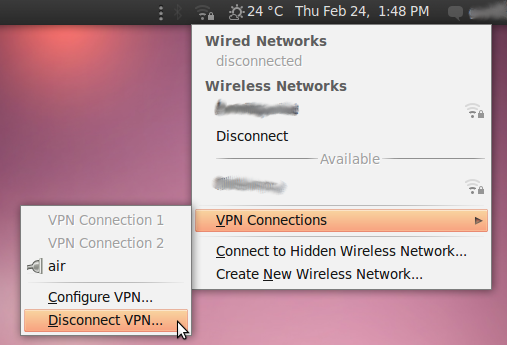
\includegraphics{vpn_ubuntu_016.png}
\caption{VPN on Ubuntu}
\end{figure}

